\chapter{How Supervised Learning Works}
\label{ch:supervised}

\chapterguide%
  {Stages 1 and 2: prepared data, basic statistics, vectors, and distance measures.}
  {Formulate regression and classification tasks, read a loss function, distinguish parametric from non-parametric models, and set up a baseline that any serious model must beat.}

Supervised learning uses examples that contain both input features $\bm{x}$ and a known target $y$. The model learns a mapping $f$ so that $f(\bm{x})$ is close to the correct target on data it has never seen. The previous chapter separated the major learning signals. We now enter the supervised branch. This chapter begins Stage 3A. It sets up the objective, loss, target types, and baseline that every supervised algorithm relies on. The next two chapters establish how supervised models are evaluated and selected without contaminating the final test set; Stage 3B begins only after that workflow is secure.

\begin{intuition}
Supervised learning is learning by example with an answer key. Someone hands the model thousands of solved problems (``this house sold for \$310{,}000'', ``this email was spam'') and the model's job is to work out the general rule connecting the inputs to the answers, so that it can solve new problems where nobody knows the answer yet.
\end{intuition}

\begin{firstread}
The entire chapter can be reduced to a loop: make a prediction, compare it with the known answer, measure the mistake, and adjust the rule. A \term{loss function} is simply the chosen mistake score. A \term{baseline} is the simple rule the model must beat.
\end{firstread}

\section{Two kinds of targets}

\begin{description}[leftmargin=1.25in,style=nextline]
  \item[Regression] The target is a number on a continuous scale: a price, a temperature, a length of stay. Predictions can be too high or too low by some amount.
  \item[Classification] The target is a category: spam or not spam, which of ten digits, which species. Predictions are right or wrong, and a good model also reports \emph{how confident} it is through class probabilities.
\end{description}

The same dataset can support either task depending on how the target is defined. Predicting tomorrow's exact temperature is regression; predicting whether tomorrow will be ``hot'' or ``cold'' is classification. Ordered categories (small, medium, large) and counts sit between the two and sometimes need special treatment, but regression and classification cover the vast majority of practical problems.

\section{The supervised-learning objective}

A training dataset can be written as
\[
  \mathcal{D}={\left\{(\bm{x}_i,y_i)\right\}}_{i=1}^{n}.
\]
The model has parameters $\bm{\theta}$ and produces predictions $\hat{y}_i=f_{\bm{\theta}}(\bm{x}_i)$. Training usually minimizes the average loss over the training set,
\[
  \hat{R}(\bm{\theta})
  =\frac{1}{n}\sum_{i=1}^{n}
  \mathcal{L}\!\left(y_i,f_{\bm{\theta}}(\bm{x}_i)\right),
\]
a quantity called the \term{empirical risk}. Reading this equation piece by piece: $\mathcal{L}$ scores one prediction against one true answer, the sum walks through every training example, and dividing by $n$ turns the total into an average. Training searches for the parameter values $\bm{\theta}$ that make this average as small as possible.

\begin{keyidea}
Training loss measures how well the model fits known examples. Validation and test metrics estimate how well it will perform on new examples. These are different things, and the entire craft of machine learning lives in that difference.
\end{keyidea}

\section{Loss functions: how wrongness is measured}

A loss function converts ``the prediction was wrong'' into a number, and the choice of number shapes what the model learns to care about.

For regression, with error $e=y-\hat{y}$, the two workhorses are
\[
  \mathcal{L}_{\text{squared}}(e)=e^2,
  \qquad
  \mathcal{L}_{\text{absolute}}(e)=|e|.
\]

\begin{mlfigure}
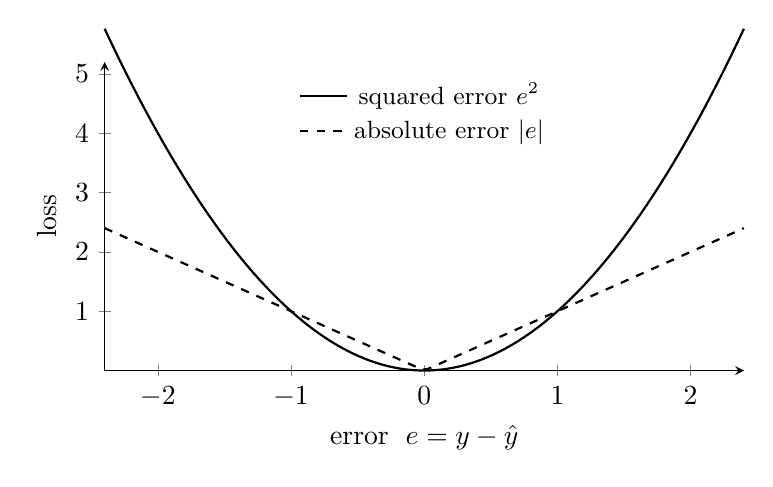
\begin{tikzpicture}
\begin{axis}[
  width=0.80\linewidth, height=5.5cm,
  axis lines=left,
  xlabel={error $\;e=y-\hat{y}$}, ylabel={loss},
  domain=-2.4:2.4, samples=100, ymin=0, ymax=5.2,
  xtick={-2,-1,0,1,2}, ytick={1,2,3,4,5},
  legend style={draw=none, font=\small, at={(0.5,0.97)}, anchor=north},
  clip=false
]
\addplot[thick] {x^2};
\addlegendentry{squared error $e^2$}
\addplot[thick, dashed] {abs(x)};
\addlegendentry{absolute error $|e|$}
\end{axis}
\end{tikzpicture}
\end{mlfigure}

\begin{intuition}
Squared error is a strict teacher: an error of $2$ costs $4$, but an error of $10$ costs $100$, so the model becomes obsessed with avoiding large mistakes --- and therefore very sensitive to outliers. Absolute error charges every unit of error the same price, so the model tolerates a few large misses in exchange for being close most of the time.
\end{intuition}

For classification, the loss that people often care about --- did the model get the label right or not, the \term{0--1 loss} --- is flat almost everywhere, which gives an optimizer no slope to follow. Practical algorithms therefore minimize tractable stand-ins instead: logistic regression uses \term{cross-entropy} (\chapref{ch:classification}), and support vector machines use the \term{hinge loss} (\chapref{ch:svm}). These surrogate losses make optimization possible, but the final model must still be judged with application-relevant metrics.

\subsection{What the loss shapes actually look like}

A loss function is a rule for turning ``how wrong were you?'' into a single number. Different rules punish mistakes differently, and that choice quietly shapes the model you end up with.

\begin{mlfigure}
\begin{tikzpicture}[baseline=(current bounding box.north)]
\begin{axis}[
  width=0.45\linewidth, height=4.8cm, axis lines=left,
  title style={font=\small\bfseries\color{MLNavy},yshift=4pt}, title={Regression losses},
  xlabel={Error $(y-\hat y)$}, ylabel={Penalty},
  label style={font=\scriptsize\color{MLMuted}}, tick label style={font=\scriptsize\color{MLMuted}},
  legend style={font=\scriptsize,draw=none,fill=white,fill opacity=0.88,
                text opacity=1,rounded corners=1pt,inner sep=2pt,
                at={(0.5,0.94)},anchor=north,legend columns=3,
                /tikz/every even column/.append style={column sep=0.7em}},
  domain=-3:3, samples=101, xmin=-3, xmax=3, ymin=0, ymax=6.5,
  ytick={0,2,4,6}
]
\addplot[MLBlue,very thick]{x^2};              \addlegendentry{squared}
\addplot[MLTeal,very thick]{abs(x)};           \addlegendentry{absolute}
\addplot[MLOrange,very thick,dashed]{abs(x)<1 ? 0.5*x^2 : abs(x)-0.5}; \addlegendentry{Huber}
\end{axis}
\end{tikzpicture}
\hfill
\begin{tikzpicture}[baseline=(current bounding box.north)]
\begin{axis}[
  width=0.45\linewidth, height=4.8cm, axis lines=left,
  title style={font=\small\bfseries\color{MLNavy},yshift=4pt}, title={Cross-entropy loss},
  xlabel={Predicted probability of the true class}, ylabel={Penalty},
  label style={font=\scriptsize\color{MLMuted}}, tick label style={font=\scriptsize\color{MLMuted}},
  domain=0.02:1, samples=101, xmin=0, xmax=1, ymin=0, ymax=4
]
\addplot[MLRed,very thick]{-ln(x)};
\node[font=\scriptsize\color{MLRed},align=center,fill=white,fill opacity=0.88,
      text opacity=1,rounded corners=0.5mm,inner sep=1.5pt]
  at (axis cs:0.43,3.2) {confident\\and wrong};
\node[font=\scriptsize\color{MLGreen},align=center,fill=white,fill opacity=0.88,
      text opacity=1,rounded corners=0.5mm,inner sep=1.5pt]
  at (axis cs:0.78,0.75) {confident\\and right};
\end{axis}
\end{tikzpicture}
\end{mlfigure}

\begin{intuition}
Squared error is a curve, so a mistake twice as large is punished four times as hard. That makes the model chase outliers. Absolute error is a straight V, so every extra unit of error costs the same, which makes it far calmer around unusual points. Huber loss is the compromise: curved near zero, straight far away.

Cross-entropy has one dramatic feature: as the predicted probability of the true answer approaches zero, the penalty runs off to infinity. Being confidently wrong is treated as almost unforgivable, which is precisely what you want from a model that reports probabilities.
\end{intuition}

\begin{keyidea}
Choose the loss to match the cost of being wrong. If one enormous error is much worse than several small ones, use squared error. If a few strange rows should not dominate the fit, use absolute error or Huber.
\end{keyidea}

\section{Parametric and non-parametric models}

\begin{mltable}
\begin{tabularx}{\linewidth}{@{}>{\bfseries\leavevmode\color{MLNavy}}p{0.21\linewidth}p{0.43\linewidth}X@{}}
\toprule
\rowcolor{MLPaleBlue!92}
Model family & Structure and examples & Trade-off \\
\midrule
Parametric models & Assume a fixed functional form with a fixed number of parameters, regardless of how much data arrives. Examples include linear regression, logistic regression, and naive Bayes. & They train fast, predict fast, and are easy to interpret, but the assumed form limits what they can express. \\
Non-parametric models & Let complexity grow with the data. Nearest neighbors keeps the entire training set; a decision tree grows as many branches as the data supports. & They can fit almost any shape of relationship, at the price of needing more data and more care to avoid overfitting. \\
\bottomrule
\end{tabularx}
\end{mltable}

Neither family is better in general. A parametric model with the right form is hard to beat on small data; a non-parametric model shines when the relationship is complicated and data is plentiful.

\section{Always start with a baseline}
\label{sec:baselines}

A \term{baseline} is the simplest prediction rule imaginable, evaluated with the same metrics and splits as any real model:

\begin{itemize}
  \item for regression, predict the training-set mean (or median) of the target for every observation;
  \item for classification, predict the most common class for every observation;
  \item when domain rules exist (``flag any transaction over \$10{,}000''), evaluate those too.
\end{itemize}

Baselines protect against two common embarrassments. First, they expose data problems: if the majority-class baseline achieves 97\% accuracy, the dataset is severely imbalanced and accuracy is the wrong metric. Second, they calibrate expectations: a complicated model that beats the mean predictor by a hair is probably not learning much, no matter how impressive its machinery.

\begin{workedexample}
In a dataset where 950 of 1{,}000 emails are legitimate, the rule ``predict \emph{not spam} for everything'' is 95\% accurate while catching zero spam. Any model claiming success must therefore show more than high accuracy --- for instance, good recall and usable precision on the rare spam class (\chapref{ch:evaluation}).
\end{workedexample}

\section{Baselines you should always run}


\begin{mlfigure}
\begin{tikzpicture}[
  node distance=0.4cm and 0.6cm,
  bx/.style={draw=MLBlue,fill=MLPaleBlue,rounded corners=1.5mm,minimum width=3.1cm,minimum height=0.95cm,align=center,font=\scriptsize\bfseries\color{MLNavy}},
  arr/.style={-{Stealth[length=2mm]},thick,draw=MLTeal}
]
\node[bx,fill=MLPaleGray,draw=MLMuted] (b0) {Baseline\\always guess the average};
\node[bx,right=of b0] (b1) {Simple model\\linear or a shallow tree};
\node[bx,right=of b1] (b2) {Stronger model\\forest or boosting};
\node[bx,right=of b2] (b3) {Tuned model\\cross-validated settings};
\draw[arr] (b0)--(b1); \draw[arr] (b1)--(b2); \draw[arr] (b2)--(b3);
\node[font=\scriptsize\itshape\color{MLMuted},below=0.05cm of b1] {stop here if it is good enough};
\end{tikzpicture}
\end{mlfigure}

\begin{analogy}
The ladder above is how experienced practitioners actually work: climb one rung at a time and stop as soon as the result is good enough for the decision at hand. Beginners tend to leap straight to the top rung, and then have no way of knowing whether the complicated model earned its complexity.
\end{analogy}

\begin{pitfall}
A model that beats the baseline by a large margin on the very first try deserves suspicion before celebration. Check for leakage: an identifier column, a feature recorded after the outcome was known, or duplicate rows spread across both the training and test sets.
\end{pitfall}

\section{A map of the algorithms ahead}

After \chapref{ch:training}, the six algorithm chapters that follow cover the supervised model families every practitioner is expected to know. They are grouped by the core idea each family is built on.

\begin{mltable}
\renewcommand{\arraystretch}{1.16}
\setlength{\tabcolsep}{5pt}
\begin{tabularx}{\linewidth}{@{}>{\footnotesize\raggedright\arraybackslash}p{0.12\linewidth}>{\footnotesize\raggedright\arraybackslash}p{0.42\linewidth}>{\footnotesize\raggedright\arraybackslash}X@{}}
\toprule
\rowcolor{MLPaleBlue!92}
\normalfont\bfseries Chapter & \bfseries Algorithms & \bfseries Core idea \\
\midrule
\ref{ch:regression} & Linear, polynomial, ridge, lasso, elastic net regression & Fit a weighted sum of features; penalize large weights \\
\ref{ch:classification} & Logistic regression, softmax, LDA, QDA, perceptron & Draw a linear boundary between classes \\
\ref{ch:knn-nb} & $k$-nearest neighbors, naive Bayes & Predict from similar examples; predict from per-feature probabilities \\
\ref{ch:decision-trees} & Decision trees (CART) & Ask a sequence of yes/no questions \\
\ref{ch:ensembles} & Bagging, random forests, AdaBoost, gradient boosting, stacking & Combine many models into one predictor \\
\ref{ch:svm} & Support vector machines, kernels, SVR & Maximize the margin; separate after mapping to a richer space \\
\bottomrule
\end{tabularx}
\end{mltable}

Each chapter follows the same rhythm: what the algorithm does in plain words, how training works step by step, a small worked example with real numbers, and finally when to use it and what its knobs (hyperparameters) control. \chapref{ch:svm} closes the supervised-learning stage with a side-by-side comparison of the models in the table.

\begin{keyidea}
All supervised algorithms answer the same question --- ``what function turns these inputs into those outputs?'' --- but they differ in the shapes of functions they can represent, the assumptions they make, and the amount of data they need. Learning the algorithms means learning those trade-offs, not memorizing formulas.
\end{keyidea}

\begin{modelcard}{Supervised Learning - Project Checklist}
\begin{tabularx}{\linewidth}{@{}>{\bfseries\leavevmode\color{MLNavy}}p{0.17\linewidth}>{\raggedright\arraybackslash}X@{}}
Question 1 & Is the target a number, a category, or a special type such as a count or ordered label? \cr
Question 2 & What simple baseline should the model beat? \cr
Question 3 & Which loss guides training, and which metric matches the real cost of mistakes? \cr
Question 4 & How will the split imitate future predictions? \cr
Question 5 & Does the final model need interpretability, probabilities, speed, or a nonlinear boundary? \cr
\end{tabularx}
\end{modelcard}

% ==== EXPANDED EDITION ADDITIONS ====

\section{Kaggle lab: compare supervised baselines fairly}
\label{sec:kaggle-titanic-supervised}

\begin{kaggleproject}{Titanic --- linear versus nonlinear classification}
\kagglesource{https://www.kaggle.com/datasets/yasserh/titanic-dataset}{Titanic Dataset}
\textbf{File.} \texttt{all\_datasets/titanic\_dataset/Titanic-Dataset.csv}\\
\textbf{Target.} \texttt{Survived}.\\
\textbf{Question.} With the same features, development split, preprocessing, and metrics, how do logistic regression and a random forest compare?\\
\textbf{Before running.} Predict which model is more flexible and why a single validation split is not enough to declare a universal winner.

\begin{labmode}
Stage 3A is still workflow-focused. Use the reference pipeline, but you are responsible for adding and interpreting the no-skill baseline.
\end{labmode}

\lstinputlisting[style=mlpython]{all_experiments/lab05-titanic_supervised_baseline.py}

\begin{tryit}
Add a \texttt{DummyClassifier(strategy="most\_frequent")} as a true no-skill baseline. Then explain what additional value logistic regression and the random forest provide over that reference.
\end{tryit}
\end{kaggleproject}




\begin{quickcheck}
\begin{enumerate}
  \item How does a regression target differ from a classification target, and what does that change about the kind of prediction produced?
  \item Why can the loss used for fitting differ from the metric used to report practical performance?
  \item What does a learned model have to demonstrate beyond beating its own training loss?
\end{enumerate}
\end{quickcheck}

\begin{chapterrecap}
\begin{itemize}
  \item Supervised learning uses feature-target pairs to learn a prediction rule.
  \item Regression predicts numbers; classification predicts categories or class probabilities.
  \item A loss guides training, while validation and test metrics estimate performance on new data.
  \item Parametric models use a fixed form; non-parametric models can grow in complexity with the data.
  \item Every serious model should be compared with a simple baseline.
\end{itemize}
\end{chapterrecap}
